\def\conf{0}
% * <themis.gouleakis@gmail.com> 2015-10-09T19:27:57.769Z:
%
% 
%
\def\icalp{0}
\def\both{0}

\documentclass[11pt]{article}
\usepackage{fullpage}


\usepackage{graphicx,amsfonts,amsmath,amssymb,epsfig,hyperref,color}
\usepackage{algorithm}
\usepackage{pdfpages}
\usepackage{enumitem}
\usepackage{multirow}
\usepackage{thm-restate}

\usepackage{mathtools}

\usepackage[noend]{algpseudocode}
\usepackage[english]{babel}
\usepackage[utf8]{inputenc}
\usepackage{amsmath}
\usepackage{graphicx}
\usepackage[colorinlistoftodos]{todonotes}

\usepackage{verbatim}
\usepackage{comment}
\usepackage{hyperref}

\usepackage{boxedminipage}
\usepackage{fullpage}
\usepackage{array}
\usepackage[normalem]{ulem}

\usepackage{relsize}
\usepackage{amsthm}

%\usepackage{amsmath,amssymb,amsthm}
%\theoremstyle{definition}
%\newtheorem{defn}{Definition}
%\newtheorem{ques}{Question}

%\theoremstyle{remark}
%\newtheorem{obs}{Observation}
%\newtheorem{rem}{Remark}

%\theoremstyle{definition}
\newtheorem{lemma}{Lemma}
\newtheorem{claim}{Claim}
\newtheorem{theorem}{Theorem}
\newtheorem{definition}{Definition}
\newtheorem{corollary}{Corollary}
\newtheorem{proposition}{Proposition}

\setlength{\parindent}{0pt}
\setlength{\parskip}{1em}

\def\ll{\left}
\def\rr{\right}
\def\RR{\mathbb{R}}
\def\ee{\mathbb{E}}
\def\pp{\mathbb{P}}
\def\bo{\mathcal{O}}
\def\Bo{\mathlarger{\mathcal{O}}}
\def\bt{\Theta}
\def\polylog{\mathrm{polylog}\;}

\DeclarePairedDelimiter\floor{\lfloor}{\rfloor}
\newcommand{\SL}[2]{\sum\limits_{#1}^{#2}}
\newcommand{\BSL}[2]{\mathlarger{\mathlarger{\sum}\limits_{#1}^{#2}}}
\newcommand{\PL}[2]{\prod\limits_{#1}^{#2}}
\newcommand{\BPL}[2]{\mathlarger{\mathlarger{\prod}\limits_{#1}^{#2}}}

\newcommand{\anak}[1]{\todo[inline,color=green]{Anak: #1}}

\renewcommand{\vec}[1]{\mathbf{#1}}

%\usepackage{hyperref}
\usepackage{multirow}

\usepackage[margin=10pt]{subfig}

\usepackage{graphicx}
\usepackage{colortbl}
\newcommand{\lemautorefname}{Lemma}
\usetikzlibrary{
  shapes.multipart,
  matrix,
  positioning,
  shapes.callouts,
  shapes.arrows,
  calc}


\title{Distributed Density Estimation} 

\date{}
\author{
Amartya Shankha Biswas
\thanks{MIT, Cambridge MA 02139.
E-mail: {\tt  asbiswas@mit.edu}.}
}


\begin{document}


\maketitle

%\section{Miscellaneous Results}
%\label{sec:miscellaneous_results}

%\section{Domino Tiling the $2\times n$ grid}
We will consider the problem of tiling a square grid with dominos.
This problem has a long history and various importtant applications in statistical physics.
Specifically, we will focus on the local generation of domino tilings of a $2\times n$ grid from the uniform distribution.
The queries will be as an index, and the generator should report the orientation of the domino at the $i^{th}$ position in the grid.
%\begin{figure}[htbp]
    %\centering
    %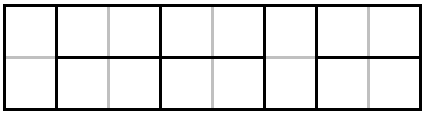
\includegraphics[width=\textwidth]{images/domino2.png}
    %\caption{}
    %\label{fig:dom2}
%\end{figure}

It is a well known result \todo{cite} that the number of tilings of a $2\times n$ grid is exactly $F_n$.
To aid with generalization, we will instead allow the generator to respond with the splitting boundary of the current tiling instead.
For example, in Figure~\ref{fig:b20}, the boundary is a vertical line at the specified position.
In Figure~\ref{fig:b21}, the boundary is horizontal, indicating that there are two horizontal dominos at that location.
Note that Figure~\ref{fig:b22} is impossible for a $2\times n$ grid.
It should be clear that this query model is equivalent.

\begin{figure}[h]
    \centering
    \begin{subfigure}[b]{0.4\textwidth}
        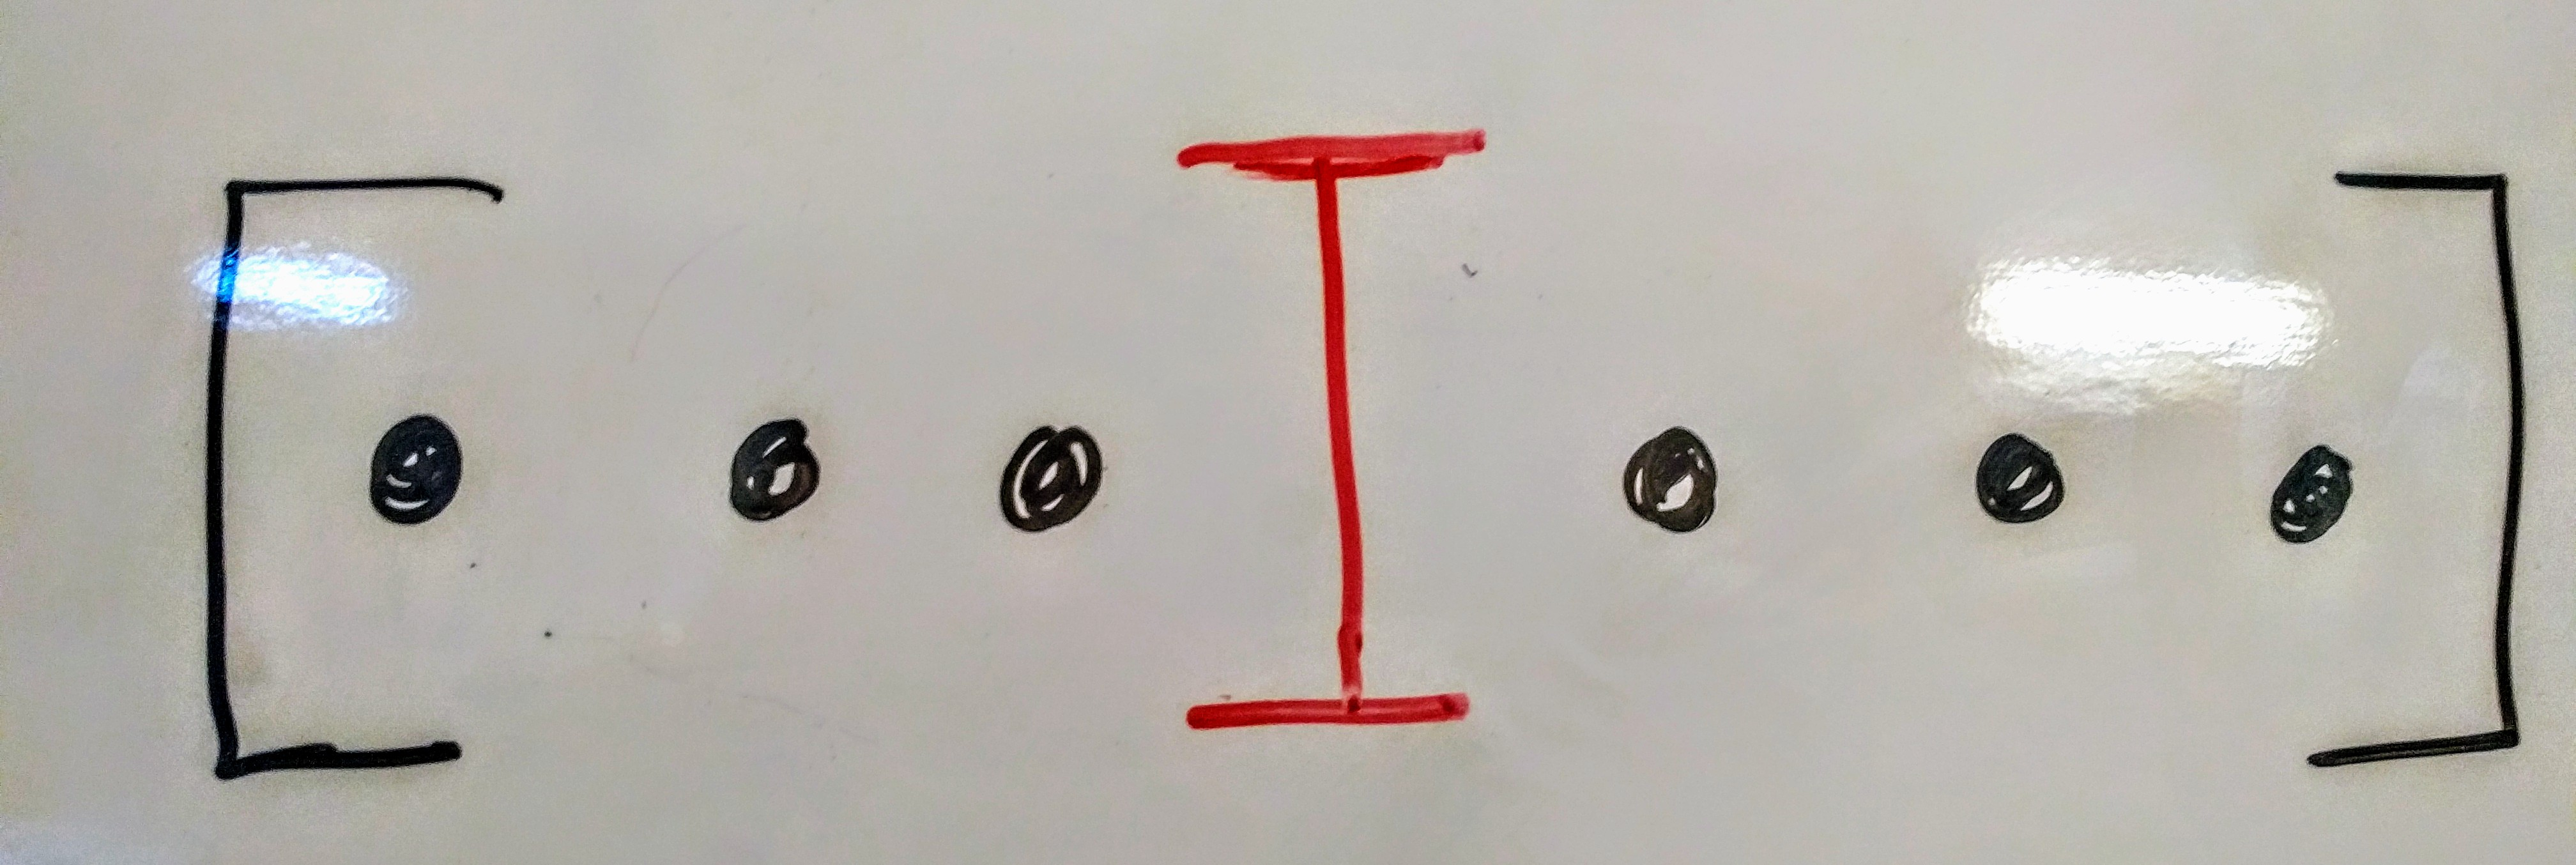
\includegraphics[width=\linewidth]{images/tile2-0.jpg}
        \label{fig:b20}
    \end{subfigure}
    \begin{subfigure}[b]{0.4\textwidth}
        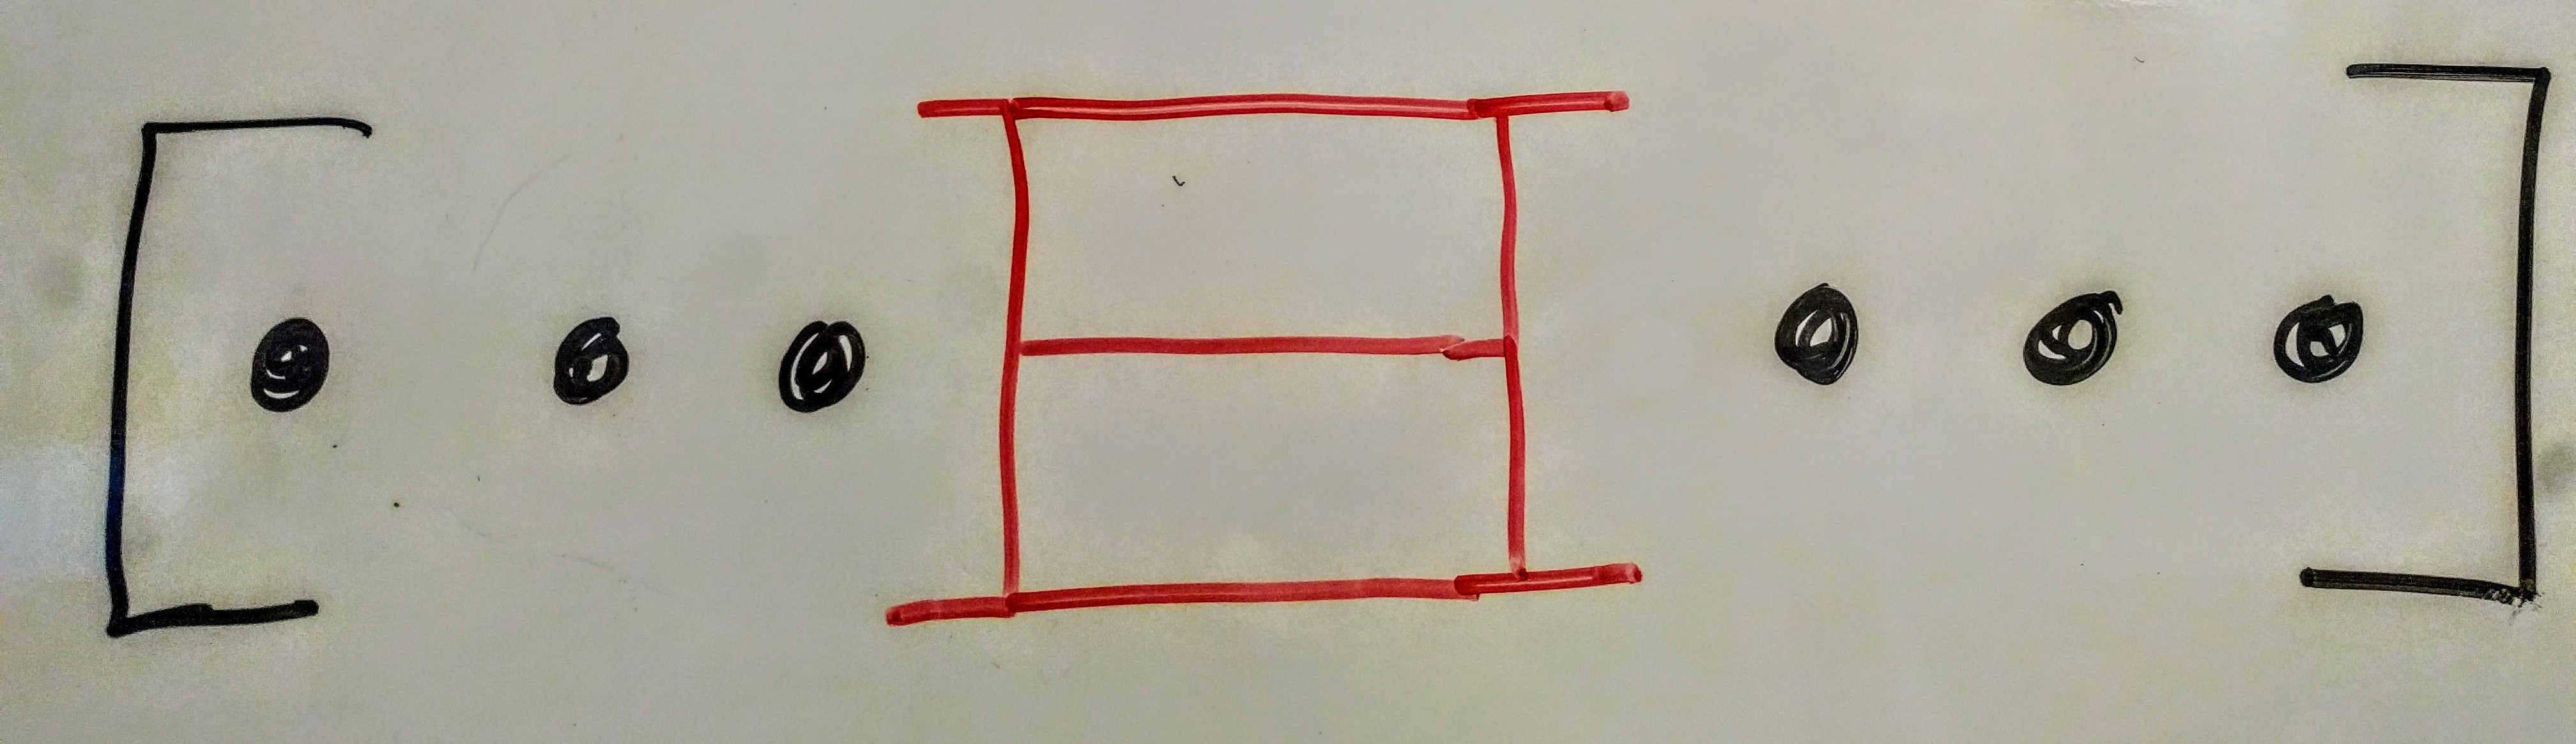
\includegraphics[width=\linewidth]{images/tile2-1.jpg}
        \label{fig:b21}
    \end{subfigure}

    \begin{subfigure}[b]{0.5\textwidth}
        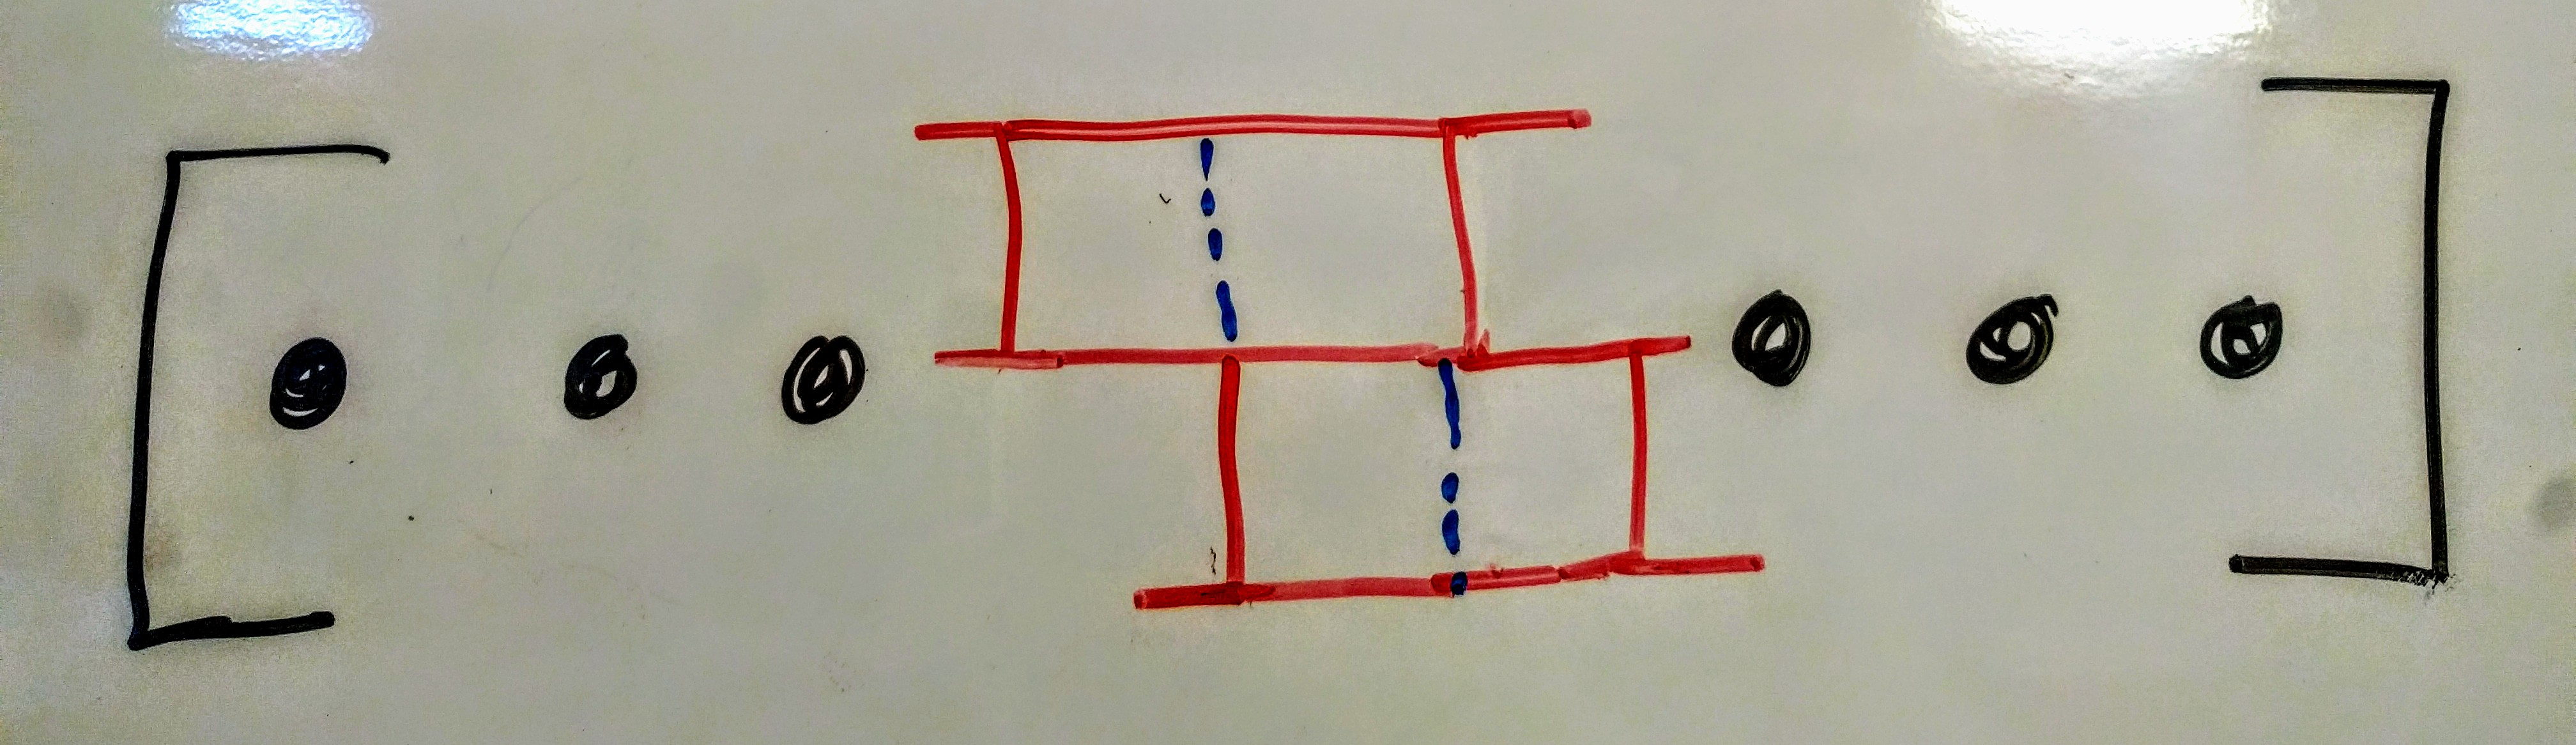
\includegraphics[width=\linewidth]{images/tile2-2.jpg}
        \label{fig:b22}
    \end{subfigure}
    \caption{Caption for this figure with two images}
    \label{fig:boundary2}
\end{figure}

Now, consider a query to the location $i$, such that all positions between $i-a$ and $i+b$ have not been queriesd so far.
So, there is a blank $2\times(a+b)$ size sub-grid that we have to sample from.
Let us consider the number of possible tilings resulting from each possible splitting boundary.
\begin{enumerate}
    \item Vertical Boundary -- This indicates that we divide the region into two sub-grids with sizes
          $2\times a$ and $2\times b$.
          So, the total number of possible tilings is exactly $F_a\cdot F_b$.
    \item Horizontal Boundary -- This indicates that we divide the region into two sub-grids with sizes
          $2\times (a-1)$ and $2\times (b-1)$.
          So, the total number of possible tilings is exactly $F_{a-1}\cdot F_{b-1}$.
\end{enumerate}

So the probabilities are computed as $\frac{F_a\cdot F_b}{F_a\cdot F_b + F_{a-1}\cdot F_{b-1}}$
and $\frac{F_{a-1}\cdot F_{b-1}}{F_a\cdot F_b + F_{a-1}\cdot F_{b-1}}$.
Now, we face the issue of approximating these fractions.
If either of the values $a$ or $b$ are less than $\Theta(\sqrt n)$,
then we can compute the exact value of the corresponding $F_a$ or $F_b$.
Otherwise, we use Lemma~\ref{lem:rat_conv} to approximate $F_a=\phi\cdot F_{a-1}$ and $F_b=\phi\cdot F_{b-1}$.
So, the probability of the vertical boundary becomes
$$
\frac{F_a\cdot F_b}{F_a\cdot F_b + F_{a-1}\cdot F_{b-1}} = \frac{\phi^2}{\phi^2+1}
$$
Similarly, the probability of a horizontal split with a top and bottom domino becomes $1/(\phi^2+1)$.
Note that this also determines the two adjacent boundaries.

The only information we needed to make this query was the extent of the un-queried interval $[i-a, i+b]$.
We can use any standard data-structure that allows insertion in positions $\{1, 2\cdots,n+1\}$,
and provides successor and predecessor queries.

Here's we can be fancy and use Van-Emde-Boas trees to get a $\Bo(\log\log n)$ query time.
However, in some cases, the exact value of a Fibonacci number still needs to be computed, and this takes $\Bo(\log n)$ time.
The faster queries only work when the new query is "far enough" ($\Bo(\log n)$ distance) away from all previous queries.



%\subsection{Permutations}

\anak{Did we try to support more information that just computing $\pi(i)$?}
[Specification]

In addition to a table (dictionary) containing all assigned values $\pi(i)$, we maintain the following binary trees,
whose nodes are generated on-the-fly in response to queries.

$T_1$: Each node of $T_1$ corresponds to a specific range of indices,
where the root represents the entire range $\{1, \ldots, N\}$,
and its two children represents each (approximately) half of the parent's range.
Each node counts the indices $i$ in the range, such that $\pi(i) = \bot$.
Initially $T_1$ only contains the root node, and the number of unassigned indices are $N$.
The children are only generated when we need to traverse down from the root; as these nodes are generated,
all of the indices in their ranges are unassigned.
Once an index becomes assigned, we simply update the information along the path in $\Bo(\log n)$ time.

$T_2$: $T_2$ is similar to $T_1$ but instead of maintaining the number of indices in the range that are still unassigned,
it maintains the number of values in the range that are still unused (have not been assigned to an index).
Similarly, we may sample an unused value or mark it as used within $\Bo(\log n)$ time.

To compute $\pi(i)$, first we check the table for $\pi(i)$ and return its value if $\pi(i)\neq\bot$.
Otherwise, sample an unused value $j$ from $T_2$ and mark that value as used.
Add $\pi(i) = j$ to the table, and mark index $i$ as used on $T_1$.

If we wish to support $\pi^{-1}(i)$, then also store the table of $\pi^{-1}(i)$.
To assign $\pi^{-1}(i)$, sample an unassigned index $j$ from $T_1$ then mark it as assigned,
add $\pi(j)=i$ and $\pi^{-1}(i)=j$ to the table, and mark the value $i$ as used on $T_2$.

\subsection{Generating Permutations with given Cyclic Structure}
We will use the technique from \cite{cyclic} to locally generate a random permutation with a given cyclic structure.
This algorithm uses two permutations $\pi$ and $\sigma$,
where $\pi$ is a uniformly random permutation and $\sigma$ is a fixed permutation with the given structure.
The resulting random permutation is formed by the composition $\pi^{-1}(\sigma(\pi(\cdot)))$.
We will generate the permutation $\pi$ as described in the previous section.;



We receive as input a list of cycle sizes \{$c_1, c_2,\cdots, c_k\}$ with the restriction that $\sum c_i = n$.
Now we need to locally generate the permutation $\sigma$ with the prescribed structure.
Define the indices $C_j = \SL{i=1}{j}c_i$ with $C_0 = 0$.
We will construct the cycle corresponding to $c_i$ as all the elements in the interval $\{c_{i-1}+1,c_{i-1}+2,\cdots,c_i\}$.

Of course we will not be computing $\sigma$ explicitly.
Instead, we will pre-compute the $C_j$ indices, and when given a query $\sigma(x)$,
we binary search amongst $C_j$ to find the cycle that $x$ belongs to.
Then we can report the value of $\sigma(x)$ accordingly.

So, we can now compose the generator oracles for $\pi$, $\sigma$, and $\pi^{-1}$ to get the full generator. 


%\section{Catalan Objects}%
\label{sec:catalan_objects}


\subsection{Dyck Paths}
\label{sub:dyck_paths}


Dyck paths are one interpretation of the Catalan numbers.
Here, we will instead consider a more general form of Dyck Paths, which correspond to numbers in the \textit{Catalan Trapezoid}.

A Dyck path can be constructed as a $1D$ random walk with $2n$ steps,
where the ends of the walk are pinned to zero (Figure~\ref{fig:dyck}).
This path also has the additional restriction that the walk can never reach negative values.
The number of possible Dyck paths is the $n^{th}$ Catalan number --
$$C_n = \frac{1}{n+1}\cdot {2n\choose n}$$
We will attempt to support queries to a uniformly random instance of a Dyck path.
Specifically, we will want to query the position of the $i^{th}$ index.

\subsection{Catalan Trapezoid}
First, we define Catalan trapezoids as presented in \cite{trap}.
Let $C_k(n,m)$ be the $(n,m)^{th}$ entry of the Catalan trapezoid of order $k$, where $C_1(n,m)$ corresponds to the Catalan triangle.

The interpretation is as follows. Consider a sequence of $n$ $(+1)$s and $m$ $(-1)$,
such that the sum of any initial sub-string is not less than $1-k$.
This means that we start our Dyck path at a height of $k-1$, and we are never allowed to cross below zero.
The total number of such paths is exactly $C_k(n,m)$.

Now, we state a result from \cite{trap} without proof
$$
C_k(n,m)=
\begin{cases}
{n+m}\choose m &0\le m<k\\
{{n+m}\choose{m}} - {{n+m}\choose{m-k}} &k\le m\le n+k-1\\
0 &m>n+k-1
\end{cases}
$$

%\section{Catalan Objects and Dyck Paths}%
\label{sec:catalan_objects}

Dyck paths are one interpretation of the Catalan numbers.
Here, we will instead consider a more general form of Dyck Paths, which correspond to numbers in the \textit{Catalan Trapezoid}.

A Dyck path can be constructed as a $2n$ step random walk on the $\mathbb Z^2$ lattice,
starting at the origin $(0,0)$ and ending at $(n, n)$ (Figure~\ref{fig:basic_dyck}).
Each step in the walk moves one unit either along the positive $x$-axis or the positive $y$-axis.
Given these restrictions, we would obtain a 1D random walk pinned to zero  on both sides.
A Dyck path also has the additional restriction that for any position $(x, y)$ on the path, $y-x > 0$
i.e. the walk is always on one side of the diagonal.

The number of possible Dyck paths is the $n^{th}$ Catalan number --
$$C_n = \frac{1}{n+1}\cdot {2n\choose n}$$
We will attempt to support queries to a uniformly random instance of a Dyck path.
Specifically, we will want to query the position of the $i^{th}$ index.

\begin{figure}[htbp]
    \centering
    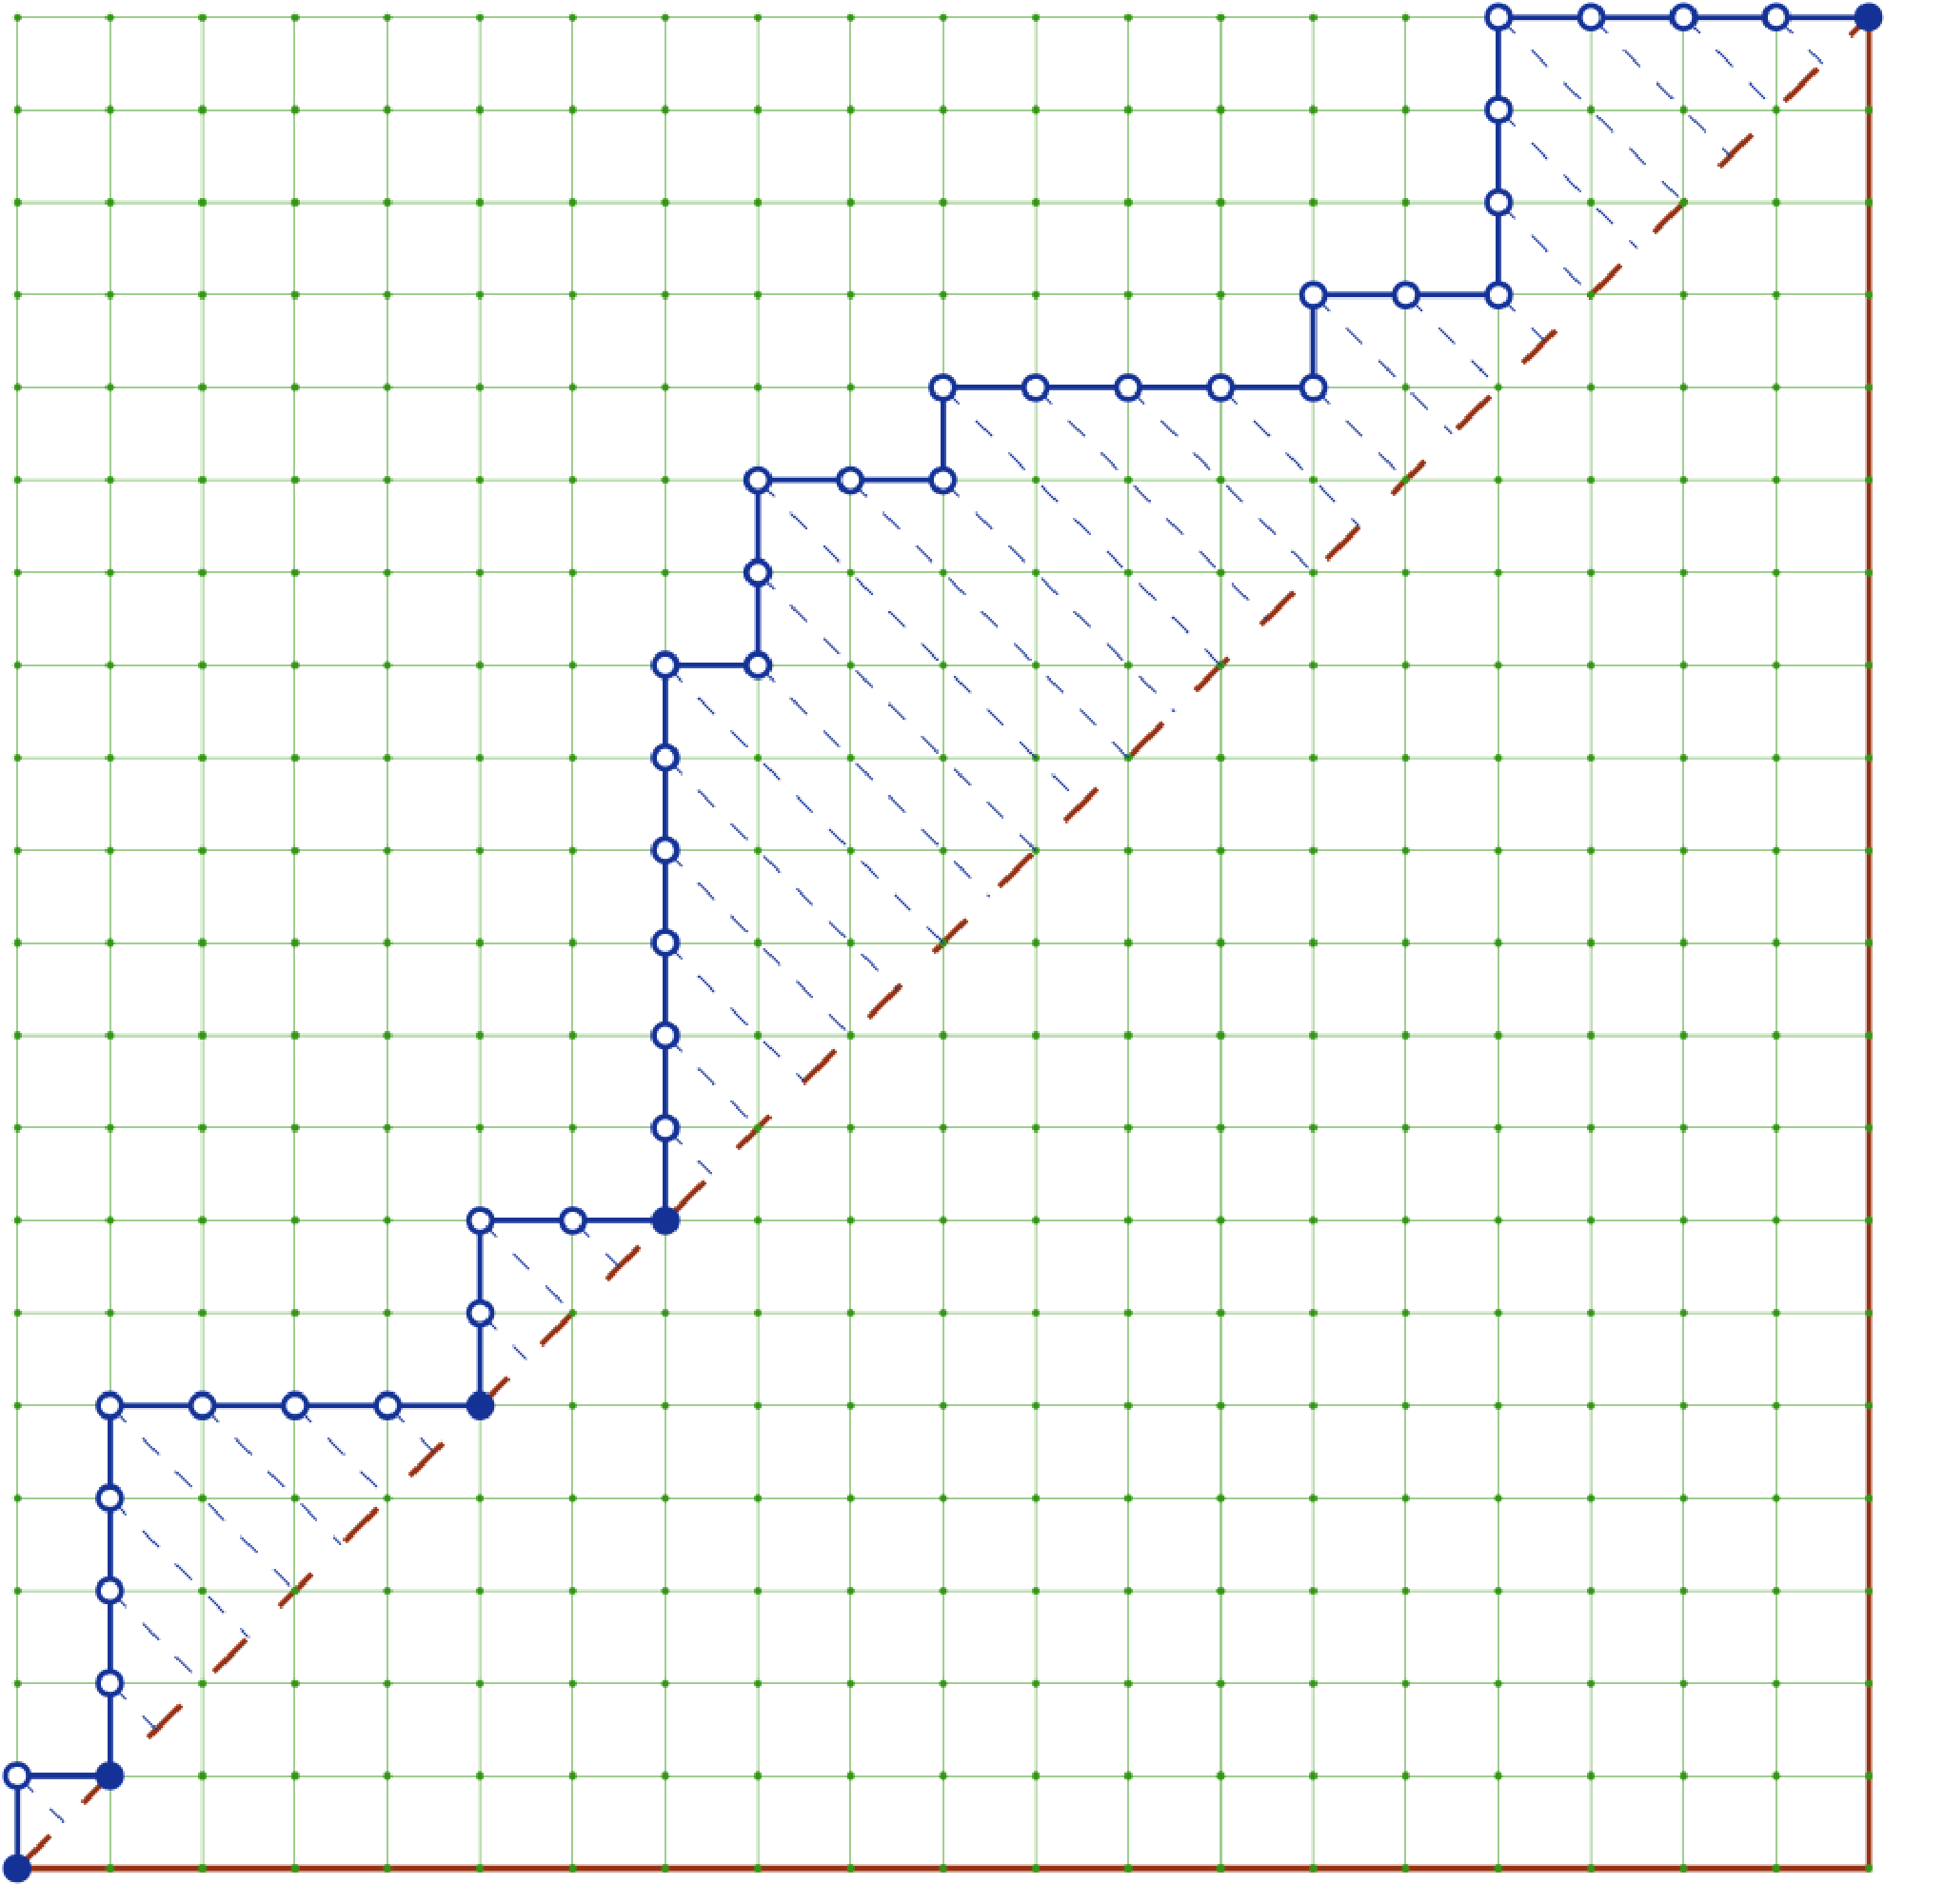
\includegraphics[width=0.7\textwidth]{dyck/basic_dyck_path.pdf}
    \caption{Simple Dyck path from $(0, 0)$ to $(20, 20)$}
    \label{fig:basic_dyck}
\end{figure}


\subsection{Catalan Trapezoids and Generalized Dyck Paths}
First, we define Catalan trapezoids as presented in \cite{trap}.
Let $C_k(n,m)$ be the $(n,m)^{th}$ entry of the Catalan trapezoid of order $k$, where $C_1(n,m)$ corresponds to the Catalan triangle.

The interpretation is as follows:
Consider a random walk from $(0,0)$ to $(m, n)$ ($n$ steps along the $y$-axis, and $m$ steps along the $x$-axis),
such that for any position $(x, y)$ along the walk, $y-x > 1-k$ (Figure~\ref{fig:complex_dyck})
i.e. the walk is always on one side of the shifted diagonal.
The total number of such paths is exactly $C_k(n,m)$.
For $k = 1$, we obtain the definition of the simple Dyck path (Figure~\ref{fig:basic_dyck}).

Now, we state a result from \cite{trap} without proof
$$
C_k(n,m)=
\begin{cases}
{n+m}\choose m &0\le m<k\\
{{n+m}\choose{m}} - {{n+m}\choose{m-k}} &k\le m\le n+k-1\\
0 &m>n+k-1
\end{cases}
$$

\begin{figure}[htbp]
    \centering
    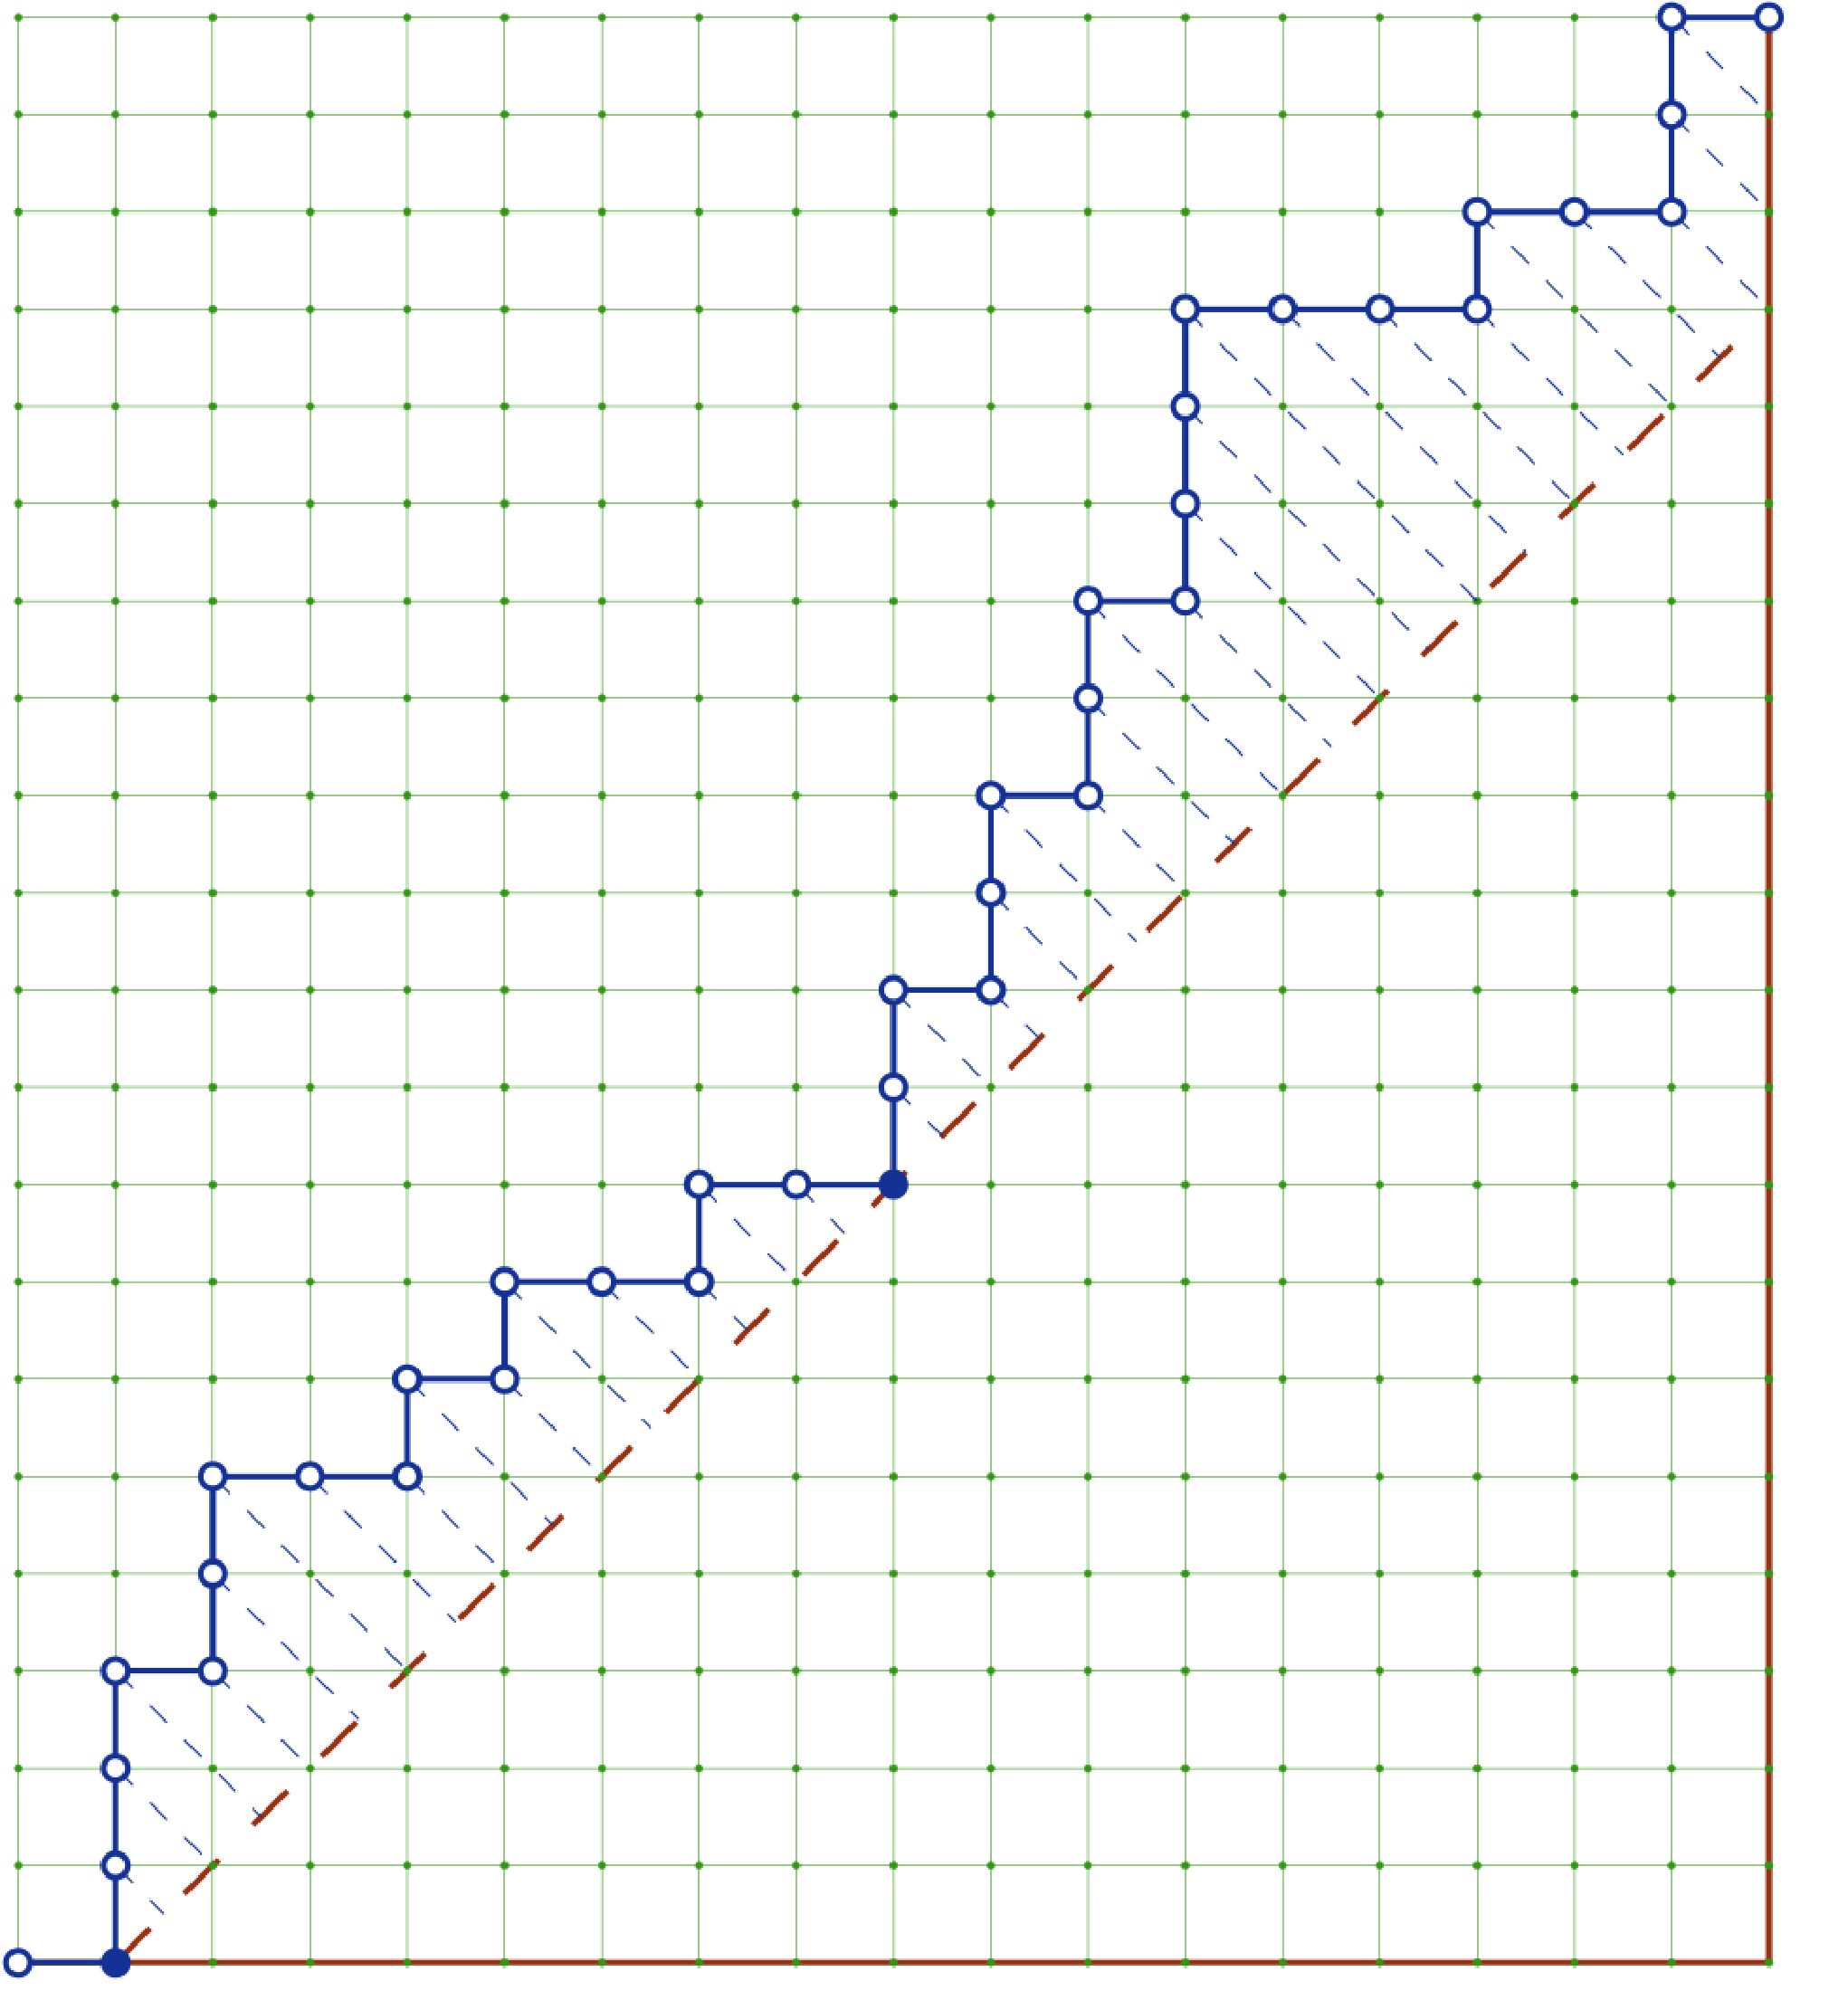
\includegraphics[width=0.7\textwidth]{dyck/complex_dyck_path.pdf}
    \caption{Complex Dyck path from $(0, 0)$ to $(18, 20)$ with $k = 2$. Notice that the diagonal is shifted.}
    \label{fig:complex_dyck}
\end{figure}

\subsection{Generating Dyck Paths}
Our general recursive step is as follows.
We consider a sequence of length $2S$ comprising of $2U$ up moves ($+1$) and $2D$ down moves ($-1$).
Additionally, the sum of any initial sequence {\color{red} prefix?} canon be less than $k-1$.
Without loss of generality, let's assume that $2D\le S$. If this were not the case,
we could simply flip the sequence and negate the elements.
This essentially means that the overall Dyck path is non-decreasing.

\begin{lemma}
$S-2D = \Bo(\log n\sqrt S) \implies U-D = \Bo(\log n\sqrt S)$
\label{lem:dyck_var0}
\end{lemma}

We want to sample the height of this path after $S$ steps.
This is the same as sampling the number of $(+1)$s that get assigned to the first half of the elements in the sequence.
We define $p_d$ as the probability that exactly $D-d$ $(-1)$s get assigned to the first half.
This means that exactly $U+d$ $(+1)$s get assigned to the first half.
Consequently, the second half will contain exactly $D+d$ $(-1)$s and $U-d$ $(+1)$s.

Let us first compute this probability.
$$
p_d = \frac{D_{left}\cdot D_{right}}{D_{tot}}
$$
Where $D_{left}$ denotes the number of valid starting sequences (first half)
and $D_{right}$ denotes the number of valid ending sequences.
Here, \textit{valid} means that each half sequence gets the appropriate number of ups and downs
and the initial sums never drop below $1-k$.
For, $D_{right}$, we will start the Dyck path from the end of the $2S$ sequence.
In this case the invalidation threshold will be a different $k'$.
This $k'$ is the final height of the $2S$ sequence. So, $k'=k+2U-2D = k+4S-2D$. We will use this fact extensively moving forward.

Also, $D_{tot}$ is the total number of possible sequences of length $2S$ , given the initial conditions.
This value is considered by constructing paths in the original direction i.e. the value of $k$ is the same.

\subsection{The Simple Case}
The problem of sampling reduces to the binomial sampling case when $k > \mathcal{O}(\log n)\sqrt S$ for some constant $c$.
In this case, the we can simply approximate the probability as
$$
\frac{{{S}\choose{D-d}}\cdot{{S}\choose{D+d}}}{{{2S}\choose{2D}}}
$$
This is because the random paths will not have initial sums less than $1-k$ with high probability.
Note that this uses the assumption that we have an increasing path.

\subsection{Path Segments Close to Zero}
The problem arises when we $k <\mathcal{O}(\log n)\sqrt{S}$. In this case we need to compute the actual probability,
Using the formula from \cite{trap}, we find that.
\begin{align}
D_{left} = {{S}\choose{D-d}}-{{S}\choose{D-d-k}} &&D_{right} = {{S}\choose{U-d}}-{{S}\choose{U-d-k'}}
\end{align}
Here, $k' = k+2U-2D$, and so $k' = \Bo(\log n)\sqrt S$.\todo{prove using Lemma~\ref{lem:dyck_var0}}

Finally, we compute the total number of Dyck paths as
$$
D_{tot} = {{2S}\choose{2D}}-{{2S}\choose{2D-k}}
$$

Now, we are going to use the following Lemma from \cite{huge}.
\begin{lemma}
\label{lem:huge}
Let $\{p_i\}$ and $\{q_i\}$ be distributions satisfying the following conditions
\begin{enumerate}
    \item There is a poly-time algorithm to approximate $p_i$ and $q_i$ up to $\pm n^{-2}$
    \item Generating an index $i$ according to $q_i$ is closely implementable.
    \item There exists a $poly(log n)$-time recognizable set $S$ such that
    \begin{itemize}
        \item $1-\SL{i\in S}{} p_i$ is negligible
        \item There exists a constant $c$ such that for every $i$, it holds that $p_i\le \log^{\mathcal{O}(1)} n\cdot q_i$
    \end{itemize}
\end{enumerate}
Then, generating an index $i$ according to the distribution $\{p_i\}$ is closely-implementable.
\end{lemma}

In this process, we will first disregard all values of $d$ where $|d|>\Theta(\sqrt S)$.
The probability mass associated with these values can be shown to be negligible \todo{bound variance of path}.

Next, we will construct an appropriate $\{q_i\}$ and show that $p_d < \log^{\mathcal{O}(1)} n\cdot q_d$
for all $|d|<\Theta(\sqrt S)$ and some constant $c$.
We will use the following distribution
$$
q_d = \frac{{S\choose D-d}\cdot{S\choose D+d}}{{2S\choose 2D}} = \frac{{S\choose D-d}\cdot{S\choose U-d}}{{2S\choose 2D}}
$$
It is shown in \cite{huge} that this distribution is closely implementable.

\begin{lemma}
First we show that $D_{left} \le \frac{c_1\cdot k}{\sqrt{S}}\cdot{{S}\choose{D-d}}$ for some constant $c_1$.
\end{lemma}
\begin{proof}
This involves some simple manipulations.
\begin{align}
D_{left} &= {{S}\choose{D-d}}-{{S}\choose{D-d-k}}\\
&= {{S}\choose{D-d}}\cdot \left[1-\frac{(D-d)(D-d-1)\cdots(D-d-k+1)}{(S-D-d+k)(S-D-d+k-1)\cdots(S-D-d+1)}\right]\\
&\le {{S}\choose{D-d}}\cdot \left[1-\left(\frac{D-d-k+1}{S-D+d+k}\right)^k\right]\\
&\le {{S}\choose{D-d}}\cdot \left[1-\left(\frac{U+d+k-(U-D+d+k-1)}{U+d+k}\right)^k\right]\\
&\le {{S}\choose{D-d}}\cdot \left[1-\left(\frac{U+d+k-\Bo(\sqrt{U})}{U+d+k}\right)^k\right]\\
&\le \frac{k}{\Theta(\sqrt{S})}\cdot{{S}\choose{D-d}}
\end{align}
\end{proof}

\begin{lemma}
Similarly, we show that $D_{right} < \frac{c_2\cdot k'}{\sqrt{S}}\cdot{{S}\choose{U-d}}$ for some constant $c_2$.
\end{lemma}
\begin{proof}
\begin{align}
D_{right} &= {{S}\choose{U-d}}-{{S}\choose{U-d-k'}}\\
&= {{S}\choose{U-d}}\cdot \left[1-\frac{(U-d)(U-d-1)\cdots(U-d-k'+1)}{(S-U-d+k')(S-U-d+k'-1)\cdots(S-U-d+1)}\right]\\
&\le {{S}\choose{U-d}}\cdot \left[1-\left(\frac{U-d-k'+1}{S-U+d+k'}\right)^{k'}\right]\\
&\le {{S}\choose{U-d}}\cdot \left[1-\left(\frac{2D-U-d-k+1}{2U-D+k+d}\right)^{k'}\right]\\
&\le {{S}\choose{U-d}}\cdot \left[1-\left(\frac{U+k+d - (2U-2D+2d+2k-1)}{U+k+d}\right)^{k'}\right]\\
&\le {{S}\choose{U-d}}\cdot \left[1-\left(\frac{U+k+d - \Bo(\sqrt U)}{U+k+d}\right)^{k'}\right]\\
&\le \frac{k'}{\Theta(\sqrt{S})}\cdot{{S}\choose{U-d}}
\end{align}
\end{proof}

Finally, we need to lower bound the value of $D_{tot}$.

\begin{lemma}
We claim that $D_{tot} < \frac{c_3\cdot k\cdot k'}{S}\cdot{{2S}\choose{2D}}$ for some constant $c_3$.
\end{lemma}
\begin{proof}
\begin{align}
D_{tot} &= {{2S}\choose{2D}}-{{2S}\choose{2D-k}}\\
&= {{2S}\choose{2D}}\cdot \left[1-\frac{(2D)(2D-1)\cdots(2D-k+1)}{(2S-2D+k)(2S-2D+k-1)\cdots(2S-2D+1)}\right]\\
&\ge {{2S}\choose{2D}}\cdot \left[1-\left(\frac{2D-k+1}{2S-2D+1}\right)^k\right]\\
&\ge {{2S}\choose{2D}}\cdot \left[1-\left(\frac{2U-(2U-2D+k-1)}{2U+1}\right)^k\right]\\
&\ge {{2S}\choose{2D}}\cdot \left[1-\left(\frac{(2U+1)-k'}{2U+1}\right)^k\right]\\
&\ge \frac{k\cdot k'}{\Theta(S)}\cdot{{2S}\choose{2D}}
\end{align}
\end{proof}

\begin{theorem}
We can now put these lemmas together to show that $p_d/q_d \le c = c_1\cdot c_2/c_3 = \Theta(1)$.
This satisfies all the conditions of Lemma~\ref{lem:huge} from \cite{huge}.
We simply need to set the accept probability less than $p_d/(c\cdot q_d)$.
\end{theorem}


%\subsection{Path Segments Close to Zero}
The problem arises when we $k <\mathcal{O}(\log n)\sqrt{S}$. In this case we need to compute the actual probability,
Using the formula from \cite{trap}, we find that.
\begin{align}
D_{left} = {{S}\choose{D-d}}-{{S}\choose{D-d-k}} &&D_{right} = {{S}\choose{U-d}}-{{S}\choose{U-d-k'}}
\end{align}
Here, $k' = k+2U-2D$, and so $k' = \Bo(\log n)\sqrt S$.\todo{prove using Lemma~\ref{lem:dyck_var0}}

Finally, we compute the total number of Dyck paths as
$$
D_{tot} = {{2S}\choose{2D}}-{{2S}\choose{2D-k}}
$$

Now, we are going to use the following Lemma from \cite{huge}.
\begin{lemma}
\label{lem:huge}
Let $\{p_i\}$ and $\{q_i\}$ be distributions satisfying the following conditions
\begin{enumerate}
    \item There is a poly-time algorithm to approximate $p_i$ and $q_i$ up to $\pm n^{-2}$
    \item Generating an index $i$ according to $q_i$ is closely implementable.
    \item There exists a $poly(log n)$-time recognizable set $S$ such that
    \begin{itemize}
        \item $1-\SL{i\in S}{} p_i$ is negligible
        \item There exists a constant $c$ such that for every $i$, it holds that $p_i\le \log^{\mathcal{O}(1)} n\cdot q_i$
    \end{itemize}
\end{enumerate}
Then, generating an index $i$ according to the distribution $\{p_i\}$ is closely-implementable.
\end{lemma}

In this process, we will first disregard all values of $d$ where $|d|>\Theta(\sqrt S)$.
The probability mass associated with these values can be shown to be negligible \todo{bound variance of path}.

Next, we will construct an appropriate $\{q_i\}$ and show that $p_d < \log^{\mathcal{O}(1)} n\cdot q_d$
for all $|d|<\Theta(\sqrt S)$ and some constant $c$.
We will use the following distribution
$$
q_d = \frac{{S\choose D-d}\cdot{S\choose D+d}}{{2S\choose 2D}} = \frac{{S\choose D-d}\cdot{S\choose U-d}}{{2S\choose 2D}}
$$
It is shown in \cite{huge} that this distribution is closely implementable.

\begin{lemma}
First we show that $D_{left} \le \frac{c_1\cdot k}{\sqrt{S}}\cdot{{S}\choose{D-d}}$ for some constant $c_1$.
\end{lemma}
\begin{proof}
This involves some simple manipulations.
\begin{align}
D_{left} &= {{S}\choose{D-d}}-{{S}\choose{D-d-k}}\\
&= {{S}\choose{D-d}}\cdot \left[1-\frac{(D-d)(D-d-1)\cdots(D-d-k+1)}{(S-D-d+k)(S-D-d+k-1)\cdots(S-D-d+1)}\right]\\
&\le {{S}\choose{D-d}}\cdot \left[1-\left(\frac{D-d-k+1}{S-D+d+k}\right)^k\right]\\
&\le {{S}\choose{D-d}}\cdot \left[1-\left(\frac{U+d+k-(U-D+d+k-1)}{U+d+k}\right)^k\right]\\
&\le {{S}\choose{D-d}}\cdot \left[1-\left(\frac{U+d+k-\Bo(\sqrt{U})}{U+d+k}\right)^k\right]\\
&\le \frac{k}{\Theta(\sqrt{S})}\cdot{{S}\choose{D-d}}
\end{align}
\end{proof}

\begin{lemma}
Similarly, we show that $D_{right} < \frac{c_2\cdot k'}{\sqrt{S}}\cdot{{S}\choose{U-d}}$ for some constant $c_2$.
\end{lemma}
\begin{proof}
\begin{align}
D_{right} &= {{S}\choose{U-d}}-{{S}\choose{U-d-k'}}\\
&= {{S}\choose{U-d}}\cdot \left[1-\frac{(U-d)(U-d-1)\cdots(U-d-k'+1)}{(S-U-d+k')(S-U-d+k'-1)\cdots(S-U-d+1)}\right]\\
&\le {{S}\choose{U-d}}\cdot \left[1-\left(\frac{U-d-k'+1}{S-U+d+k'}\right)^{k'}\right]\\
&\le {{S}\choose{U-d}}\cdot \left[1-\left(\frac{2D-U-d-k+1}{2U-D+k+d}\right)^{k'}\right]\\
&\le {{S}\choose{U-d}}\cdot \left[1-\left(\frac{U+k+d - (2U-2D+2d+2k-1)}{U+k+d}\right)^{k'}\right]\\
&\le {{S}\choose{U-d}}\cdot \left[1-\left(\frac{U+k+d - \Bo(\sqrt U)}{U+k+d}\right)^{k'}\right]\\
&\le \frac{k'}{\Theta(\sqrt{S})}\cdot{{S}\choose{U-d}}
\end{align}
\end{proof}

Finally, we need to lower bound the value of $D_{tot}$.

\begin{lemma}
We claim that $D_{tot} < \frac{c_3\cdot k\cdot k'}{S}\cdot{{2S}\choose{2D}}$ for some constant $c_3$.
\end{lemma}
\begin{proof}
\begin{align}
D_{tot} &= {{2S}\choose{2D}}-{{2S}\choose{2D-k}}\\
&= {{2S}\choose{2D}}\cdot \left[1-\frac{(2D)(2D-1)\cdots(2D-k+1)}{(2S-2D+k)(2S-2D+k-1)\cdots(2S-2D+1)}\right]\\
&\ge {{2S}\choose{2D}}\cdot \left[1-\left(\frac{2D-k+1}{2S-2D+1}\right)^k\right]\\
&\ge {{2S}\choose{2D}}\cdot \left[1-\left(\frac{2U-(2U-2D+k-1)}{2U+1}\right)^k\right]\\
&\ge {{2S}\choose{2D}}\cdot \left[1-\left(\frac{(2U+1)-k'}{2U+1}\right)^k\right]\\
&\ge \frac{k\cdot k'}{\Theta(S)}\cdot{{2S}\choose{2D}}
\end{align}
\end{proof}

\begin{theorem}
We can now put these lemmas together to show that $p_d/q_d \le c = c_1\cdot c_2/c_3 = \Theta(1)$.
This satisfies all the conditions of Lemma~\ref{lem:huge} from \cite{huge}.
We simply need to set the accept probability less than $p_d/(c\cdot q_d)$.
\end{theorem}


\section{Random Coloring of a Graph}%
\label{sec:random_coloring_of_a_graph}

\todo{Query access}
We wish to locally sample an uniformly random coloring of a graph.
A $q$-coloring of a graph $G = (V, E)$ is a function $\sigma : V\rightarrow [q]$,
such that for all $(u,v)\in E$, $\sigma_u \not= \sigma_v$.
We will consider only bounded degree graphs, i.e. graphs with max degree $\le \Delta$.
Otherwise, the coloring problem becomes NP-hard\todo{cite}.

Using the technique of path-coupling, Vigoda \todo{cite} showed that for $q > 2\Delta$,
one can sample an uniformly random coloring by using a MCMC algorithm.

The Markov Chain proceeds in $T$ steps. The state of the chain at time $t$ is given by $\vec X^t\in [q]^{|V|}$.
Specifically, the color of vertex $v$ at step $t$ is $\vec X^t_v$.

In each step of the Markov process, a pair $(v, c)\in V\times [q]$ is sampled uniformly at random.
Subsequently, if the recoloring of vertex $v$ with color $c$ does not result in a conflict with $v$'s neighbors,
i.e. $c\not\in \left\{ X^t_u : u\in \Gamma(v)\right\}$, then the vertex is recolored i.e. $X_v^{t+1}\leftarrow c$.

After running the MC for $T = \mathcal{O}(n\log n)$ steps we reach the stationary distribution ($\epsilon$ close),
and the coloring is an uniformly random one.

\textbf{Exact Bound:}
$t_{mix}(\epsilon) \le \left( \frac{q-\Delta}{q-2\Delta}\right)n\left( \log n + \log(1/\epsilon)\right)$
\todo{cite book (Peres, Lyons)}



\subsection{Modified Glauber Dynamics}%
\label{sec:modified_glauber_dynamics}

Now we define a modified Markov Chain as a special case of the \emph{Local Glauber Dynamics} presented in \cite{mohsen}.
The modified Markov chain procceds in epochs.
We denote the initial coloring of the graph by $\vec X^0$ and the state of the coloring after the $k^{th}$ epoch by $\vec X^k$.
In the $k^{th}$ epoch $\mathcal E_k$:
\begin{itemize}
    \item Sample $|V|$ colors $ \langle c_1, c_2,\cdots, c_n \rangle$ from $[q]$, where $c_v$ is the proposed color for vertex $v$.
    \item For each vertex $v$, we set $\vec X^k_v$ to $c_v$ if for all neighbors $w$ of $v$, $\vec X^k_w\not=c_v$ and $\vec X^{k-1}_w\not=c_v$.
\end{itemize}
%\begin{itemize}
    %\item Pick a random permutation $\pi^{(i)}$ of the vertices $V$.
    %\item Sample $n = |V|$ colors $ \langle c_1, c_2,\cdots, c_n \rangle$ from $[q]$.
    %\item Perform the standard update using the pairs $\left\langle (\pi^{(i)}_1, c_1), (\pi^{(i)}_2, c_2), \cdots, (\pi^{(i)}_n, c_n)\right\rangle$.
%\end{itemize}

This procedure is a special case of the \emph{Local Glauber Dynamics} presented in \cite{mohsen}.
The goal in \cite{mohsen} is to find a simultaneous update rule that causes few conflicts among neighbors (and converges to the correct distribution).
Notice that we \emph{can} have adjacent nodes update in the same epoch.
However for the sake of succinctness we use their update rule and avoid a tedious path coupling argument.

\todo{Cite Path Coupling}

We can directly use the path coupling argument from \cite{mohsen} which be briefly describe below.
Given two colorings $\vec X$ and $\vec Y$, we define $d(\vec X,\vec Y)$ as the number of vertices $v$ such that $\vec X_v\not= \vec Y_v$.
We define the coupling $(\vec X,\vec Y)\rightarrow(\vec X',\vec Y')$ where $\vec X$ and $\vec Y$
differ only at a single vertex $v$ such that $\vec X_v = c_X$ and $\vec Y_v = c_Y$.
Now, we pick a random permutation of the vertices along with uniformly sampled colors:
\[
\left\langle (v_1, c_1), (v_2, c_2), \cdots, (v_n, c_n)\right\rangle
= \left\langle (\pi_1, c_1), (\pi_2, c_2), \cdots, (\pi_n, c_n)\right\rangle
\]
Now, for each $(v_i, c_i)$ in order, we update the coloring of $X$ and $Y$ as follows:
\begin{itemize}
    \item If the current color of $v_i$ as well as $c_i$ are both in $\{c_X,c_Y\}$,
    then the $\vec X$ chain picks the color $c_i$ and the $\vec Y$ chain picks the other color.
    \item Otherwise, both chains pick the same color $c_i$ for the vertex $v_i$.
\end{itemize}
We use the following result from \cite{mohsen} that bounds the coupled distance.
\begin{lemma}
\label{lem:mohsen_single_epoch_distance}
If $q = 2\alpha\Delta$ and $d(\vec X, \vec Y) = 1$,
then $\mathbb E[d(\vec X',\vec Y')] \le 1-\left( 1-\frac1{2\alpha}\right)e^{-3/\alpha} + \frac{1/2\alpha}{1-1/\alpha}$
\end{lemma}
\begin{corollary}
\label{cor:single_epoch_distansce}
If $q \ge 9\Delta$ and $d(\vec X, \vec Y) = 1$, then $\mathbb E[d(\vec X',\vec Y')] < \frac1{e^{1/3}}$
\end{corollary}

\begin{theorem}
\label{thm:modified_mixing_time}
If $q\ge 9\Delta$, then the chain is mixed after $\tau_{mix}(\epsilon) = 3\left( \ln n + \ln(\frac1{\epsilon})\right)$ epochs.
\end{theorem}
\begin{proof}
Starting for a maximum distance of $n$, the distance decreases to $1$ after at most $3\ln n$ epochs,
and it takes a further $3\ln\left( \frac{1}{\epsilon} \right)$ to reduce the distance to $\epsilon$.
\end{proof}




\subsection{Local Coloring Algorithm}%
\label{sec:local_coloring_algortihm}
Given query access to the adjacency matrix of a graph $G$ with maximum degree $\Delta$ and a vertex $v$,
the algorithm has to output the color of $v$ after running $t = \mathcal O(\ln n)$ epochs of \emph{Modified Glauber Dynamics}.
We will define the number of colors as $q = 2\alpha\Delta$ where $\alpha > 1$.

The proposals at each epoch are a vector of color samples $\vec C^{t} \thicksim_{\mathcal U} [q]^n$,
where $\vec C^t_v$ is the color proposed by $v$ in the $t^{th}$ epoch.
Note that these values are fully independent and as such any $\vec C^t_v$ can be sampled trivially.
We also use $\vec X^t$ to denote the final vector of vertex colors at the end of the $t^{th}$ epoch.
Finally, we define indicator variables $\bm \chi^t_v$ to denote if the color $\vec C^t_v$ proposed by vertex $v$ was accepted at the $t^{th}$ epoch;
$\bm \chi^t_v = 1$ if and only if for all neighbors $w\in \Gamma(v)$,
we satisfy the condition $\vec C^t_v\not= \vec X^{t-1}_w$ and $\vec C^t_v\not= \vec C^t_w$.
So, the color of a vertex $v$ after the $t^{th}$ epoch $\vec X^t_v$ is set to be $\vec C^i_v$
where $i\le t$ is the largest index such that $\bm \chi^i_v=1$.
While the proposals $\vec C^t_v$ are easy to sample, it is much less clear how we can sample the $\bm \chi^t_v$ values.
Note that we can compute $\vec X^t_v$ quite easily if we know the values $\bm\chi^i_v$ for all $i\le t$.
So, we focus our attention on the query $\func{Accepted}(v,t)$ that returns $\bm\chi^t_v$.


\subsubsection{Naive Coloring Implementations}%
\label{sec:naive_coloring_implementations}
The general strategy to sample $\bm\chi^t_v$ is to iterate over all neighbors $w$ of $v$,
and for each of them check if they conflict with $v$'s proposed color in the $t^{th}$ epoch.
Given a neighbor $w$, one naive way to do this is to iterate backwards from epoch $t$ querying to find if $w$'s proposal was accepted
until the first accepted proposal (from the latest epoch $t' < t$) is found.
At this point, if $\vec C^{t'}_w =\vec C^t_v$, then the current color of $w$ conflicts with $v$'s proposal.
Otherwise there is no conflict and we can proceed to the next neighbor.
However, this process potentially makes $\Delta$ recursive calls to a sub-problem that is only slightly smaller i.e. $T(t) \le \Delta\cdot T(t-1)$.
This leads to a running time upper bound of $\Delta^{t}$ which is superlinear for the desired mixing time $t = \Omega(\log n)$.

We can prune the number of recursive calls by only processing the neighbors $w$ which actually proposed the color $\vec C^t_v$ during \emph{some} epoch.
In this case, the expected number of neighbors that have to be probed recursively is $\le t\Delta/q$
(since the total number of neighbor proposals over $t$ epochs is at most $t\Delta$).
So, the overall runtime is upper bounded by $(t\Delta/q)^{t}$.
For this algorithm, if we allow $q > t\Delta = \Omega(\Delta\log n)$ colors, the runtime becomes sublinear.
This lower bound on $q$ is however asymptotically worse that the sequential requirement $q > 2\Delta = \mathcal O(\Delta)$.


\subsubsection{Jumping Back to Past Epochs}
\label{sec:jumping_back_to_past_epochs}
\begin{wrapfigure}[19]{r}{0.48\textwidth}
\vspace{-1.5em}
\begin{framed}
    \renewcommand\figurename{Algorithm}
    \caption{Generator}
    \label{alg:coloring}
    \begin{algorithmic}[1]
        \Procedure{Accepted}{$v, t$}
            \State {$c\gets\vec C^t_v$}
            \For{$w \gets \Gamma(v)$}
                \If {$\vec C_w^t = c$}
                    \State \Return 0
                \EndIf
                \For{$t' \gets [t, t-1, t-2, \cdots, 1]$}
                    \If {$\mathcal\vec C^{t'}_w = c$ \textbf{and} \func{Accepted}($w, t'$)}
                        \State $flag\gets \ONE$
                        \While{$t' < t-1$}
                            \State $t'\gets t' + 1$
                            \If {\func{Accepted}($w, t'$)}
                                \State $flag\gets \ZERO$
                                \State \textbf{break}
                            \EndIf
                        \EndWhile
                        \If {$flag = \ONE$}
                            \State \Return $\ZERO$
                        \EndIf
                        \State \textbf{break}
                   \EndIf
                \EndFor
            \EndFor
            \State \Return $\ONE$
        \EndProcedure
    \end{algorithmic}
\end{framed}
\end{wrapfigure}
The expected number of neighbors that need to be checked can always be $t\Delta$ in the worst case.
The crucial observation is that even though these recursive calls seem unavoidable,
we can aim to reduce the size of the recursive sub-problem and thus bound the number of levels of recursion.
Because of the more complex structure of this epoch jumping process, the main challenge is to analyze the runtime.

Algorithm~\ref{alg:coloring} shows our final procedure for sampling $\bm\chi^t_v$ where $c =\vec C^t_v$ is the color proposed by $v$ in epoch $t$.
As before, we iterate through all neighbors $w$ of $v$.
The condition $c\not=\vec C^t_w$ is can easily be checked by sampling $\vec C^t_w$ in the current epoch.
If no conflict is seen, the next step is to check whether $c\not= \vec X^{t-1}_w$.

To achieve this, we iterate through all the epochs in reverse order (without making recursive calls)
to check whether the color $c$ was ever proposed for vertex $w$.
If not, we can ignore $w$, and otherwise let's say that the last proposal for $c$ was at epoch $t'$ i.e. $\vec C^{t'}_w = c$.
Now, we directly ``jump'' to the $t'^{th}$ epoch and recursively check if this proposal was accepted.
If the proposal $\vec C^{t'}_w$ was not accepted, we keep iterating back until we find another epoch when $c$ was proposed $w$, or we run out of epochs.
Otherwise if $c$ was accepted i.e. $\bm\chi^{t'}_w = 1$,
we successively consider epochs $t'+1, t'+2, t'+3, \cdots, t-1$ to see whether the color $c$ was replaced by an accepted proposal in a future epoch,
by recursively invoking $\func{Accepted}(w,t'+i)$ in order to sample $\bm\chi^{t'+i}_w$.
At this point we have seen that $\bm\chi^{t'}_w = 1$ (color $c$ was accepted) and every subsequent proposal until the current epoch was rejected,
implying that color $c$ \emph{survived}, i.e. $\vec X^{t-1}_w = c$.
This leads to a conflict with $v$'s current proposal for color $c$ and hence $\bm\chi^t_v = 0$.
If at any of the iterations, we see that a different proposal was accepted, then $w$ does not cause a conflict and we can move on to the next neighbor.
If we exhaust all the neighbors and don't find any conflicts then $\bm\chi^t_v = 1$.

Now we analyze the runtime of $\func{Accepted}$ by constructing and solving a recurrence relation.
We will use the following lemma to evaluate the expectation of products of relevant random variables.

\begin{lemma}
\label{lem:color_reject_probability}
The probability that any given proposal is rejected $\mathbb P[\bm\chi^t_v=0]$ is at most $1/\alpha$.
Moreover, this upper bound holds even if we condition on all the values in $\vec C$ except $\vec C^t_v$.
\end{lemma}
\begin{proof}
A rejection can occur due to a conflict with at most $2\Delta$ possible values in $\{\vec C^t_w, X^{t-1}_w | w\in\Gamma(v)\}$.
Since there are $2\alpha\Delta$ colors, the rejection probability is at most $1/\alpha$.
\end{proof}

\begin{definition}
\label{def:coloring_recursions}
We define $T_t$ to be a random variable indicating the number of recursive calls performed during the execution of $\func{Accepted}(v,t)$
while sampling a single $\bm \chi_v^t$.
\end{definition}
So, the number of probes required to check whether a color $c$ (assigned at epoch $t'$) was overwritten at some epoch before $t$ is:
\begin{align}
\label{eq:color_overwrite}
\Biggl[T_{t'+1} + \mathcal B\left(\frac{1}{\alpha}\right)\cdot T_{t'+2}
+ \mathcal B\left(\frac{1}{\alpha^2}\right)\cdot T_{t'+3} + \cdots
+ \mathcal B\left(\frac{1}{\alpha^{t-t'-2}}\right)\cdot T_{t-1} \Biggr]
\end{align}

\begin{lemma}
\label{lem:coloring_recurrence}
\todo{Given graph G and q colors ...}
For $\alpha > 4.5$, the expected number of recursive calls to the procedure $\func{Accepted}$ while sampling a single $\bm\chi^t_v$
is $\mathbb E[T_t] = \mathcal{O}\left(e^{1.02t/\alpha}\right)$.
\end{lemma}
\begin{proof}
We start with the recurrence for the expected number of probes to $\{\bm\chi^{t'}\}_{t'\in[t]}$
(equivalently calls to $\func{Accepted}$) used by the algorithm.
We will use $\mathcal B(p)$ to refer to the Bernoulli random variable with bias $p$.
When checking a single neighbor $w$, the algorithm iterates through all the epochs $t'$ such that $\vec C^{t'}_w = c$
(in reality, only the last occurence matters, but we are looking for an upper bound).
If such a $t'$ is found (this happens with probability $1/q$ independently for each trial), there is one recursive call to $T_{t'}$.
Regardless of what happens, let's say the algorithm queries $T_{t'+1}, T_{t'+2}, \cdots, T_{t-1}$ until an $\func{Accepted}$ proposal is found.
Adding an extra $T_{t'}$ term to Equation~\ref{eq:color_overwrite} and summing up over all neighbors and epochs we get the following:
\begin{align}
T_{t} &\le \Delta \cdot \mathlarger\sum\limits_{t'=1}^{t} \mathbb P[C^{t'}_w = c]\cdot
\Biggl[ T_{t'} + T_{t'+1} + \mathcal B\left(\frac{1}{\alpha}\right)\cdot T_{t'+2}
+ \mathcal B\left(\frac{1}{\alpha^2}\right)\cdot T_{t'+3} + \cdots\\
&\hspace{23em}
\cdots + \mathcal B\left(\frac{1}{\alpha^{t-t'-2}}\right)\cdot T_{t-1} \Biggr]\\
&\le \Delta\cdot\mathcal B\left( \frac{1}{q}\right) \Biggl[
\mathlarger\sum\limits_{t'=1}^{t-1} T_{t'} +
\mathlarger\sum\limits_{t'=1}^{t-1} T_{t'}\cdot \left(1 + \mathcal B\left(\frac1\alpha\right) + \mathcal B\left(\frac1{\alpha^2}\right) + \cdots\right)
\Biggr]
\end{align}
In the second step, we just group all the terms from the same epoch together.
Using Lemma~\ref{lem:color_reject_probability} and the fact that $\mathbb P[C^{t'}_w = c]$ is independent of all other events,
we can write a recurrence for the expected number of probes.
\begin{align}
\mathbb E[T_t] \le \Delta\cdot\frac{1}{2\alpha\Delta}
\left[
\mathlarger\sum\limits_{t'=1}^{t-1} T_{t'} + \mathlarger\sum\limits_{t'=1}^{t-1} T_{t'}\cdot \left(1 + \frac1\alpha + \frac1{\alpha^2} + \cdots\right)
\right]
\le \frac{1}{2\alpha}\cdot \mathlarger\sum\limits_{t'=1}^{t-1} T_{t'}\cdot \left[1 + \frac{\alpha}{\alpha-1} \right]
\end{align}
Now, we make the assumption that $\mathbb E[T_{t'}]\le e^{\hagu t/\alpha}$,
and show that this satisfies the expectation recurrence for the desired value of $k$.
First, we sum the geometric series:
\[
\mathlarger\sum\limits_{t'=1}^{t-1} \mathbb E[T_{t'}] = \mathlarger\sum\limits_{t'=1}^{t-1} e^{\hagu t'/\alpha}
< \frac{e^{\hagu t/\alpha}-1}{e^{\hagu/\alpha}-1} < \frac{e^{\hagu t/\alpha}}{e^{\hagu/\alpha}-1}
\]
The expectation recurrence to be satisfied then becomes:
\[
\mathbb E[T_t]\le \frac 1{2\alpha}\cdot \frac{e^{\hagu t/\alpha}}{e^{\hagu/\alpha}-1}\cdot \left[ 1+ \frac{\alpha}{\alpha-1} \right]
= e^{\hagu t/\alpha}\cdot \frac{2\alpha-1}{2\alpha(\alpha-1)(e^{\hagu/\alpha}-1)} = e^{\hagu t/\alpha}\cdot f(\alpha, k)
\]
We notice that for $k=1.02$ and $\alpha > 4.5$, $f(\alpha) < 1$.
This can easily be verified by checking that $f(\alpha,1.02)$ decreases monotonically with $\alpha$ in the range $\alpha > 4.5$.
Thus, our recurrence is satisfied for $k=1.02$, and therefore the expected number of calls is $\mathcal O(e^{1.02t/\alpha})$.

Finally, we note that each probe potentially takes time $\mathcal O(t\Delta)$ to iterate through all the neighbors in all epochs
resulting in a total runtime of $\mathcal O(t\Delta e^{\hagu t/\alpha})$.
\end{proof}

%\begin{corollary}
%\label{cor:coloring_improved_probes}
%Instead of looking through all the epochs in order, we can use the coloring generator \todo{where?} to find the locations directly.
%\end{corollary}

\begin{theorem}
\label{thm:coloring_generator_main}
\todo{probes?}
Given adjacency list query access to a graph with $n$ nodes, maximum degree $\Delta$, and $q=2\alpha\Delta \ge 9\Delta$ colors,
we can sample the color of any given node in an ($1/n$-approximate) uniformly random coloring of the graph in a consistent manner
using only $\mathcal O(n^{6.12/\alpha}\Delta\log n)$ time space and random bits.
This is sublinear for $\alpha > 6.12$ and the sampled coloring is $1/n$-close to the uniform distribution in $L_1$ distance.
\end{theorem}
\begin{proof}
We compute the mixing time from Theorem~\ref{thm:modified_mixing_time} to obtain $\tau_{mix}(1/n) = 6\ln n$ (this is valid since $q > 9\Delta$).
Since $\alpha > 4.5$, we can invoke Lemma~\ref{lem:coloring_recurrence} to conclude that
the number of calls to $\func{Accepted}$ is $\mathcal O(n^{6.12/\alpha}\Delta\log n)$  which is sublinear for $\alpha > 6.12$.
Each call to $\func{Accepted}(v,t)$ potentially spends $t\Delta$ time looking for neighbors in each epoch before $t$.
Since $t \le 6\ln n$, the overall runtime becomes $\mathcal O(n^{6.12/\alpha}\Delta\log n)$.
\end{proof}




\bibliographystyle{alpha}

\bibliography{bib}


\end{document}
